\begin{frame}
\frametitle{Our machines are classical}
\begin{columns}
  \begin{column}{0.6\textwidth}
    \begin{figure}
    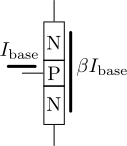
\includegraphics{transistor.pdf}
    \caption*{$\beta$ and transistor-ness depend on quantum mechanics, i.e. Fermi-Dirac distribution.}
    \end{figure}
  \end{column}
  \pause
  \begin{column}{0.4\textwidth}
    \begin{figure}
    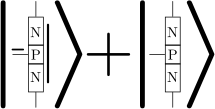
\includegraphics[scale=0.7]{transistor_superposition.pdf}
    \caption*{Quantum superposition of transistor states.}
    \end{figure}
  \end{column}
\end{columns}

\begin{itemize}
\item There's quantum mechanics under the hood, but...
\item the degrees of freedom carrying information are classical.

\end{itemize}
\end{frame}
